\section{Technologie Stack}

Eine zentrale Anforderung an das System ist die konsistente und verzögerungsfreie Darstellung eines Dokuments auf mehreren Klienten.
Die Wahl eines geeigneten Kommunikationsprotokolls ist die Grundlage für eine erfolgreiche Lösung.

Wir verwenden HTTP-Event Streams als Grundlage für die Kommunikation zwischen dem Backend Server und den Klienten.
Als konkrete Implementation dieser Technologie setzen wir Spring-WebFlux ein.
Die weitere Technologieauswahl orientiert sich an diesem Grundsatz Entscheid.

\subsection{Lösungsstrategie}
Um die verteilte Dokumentenbearbeitung zu ermöglichen, verwenden wir eine Variante des Command Patterns als Lösungsansatz.
Dabei sollen die eingehenden Änderungen am Dokument als einzelne Commands modelliert werden.
Die eingehenden Commands werden vom Backend verarbeitet und an alle Teilnehmer weitergeleitet.
Konflikte werden dabei auf dem Server gelöst.
Wenn nötig werden dabei zusätzliche Commands generiert, welche die Konflikte auflösen.


\subsection{Backend Server}
Spring WebFlux ist integriert in das Spring Boot Ökosystem und benötigt daher eine zugrundeliegende JVM\@.
Sprachen die auf der JVM aufbauen, haben den Vorteil, dass sie System Interoperabel sind.

Anstatt Java setzen wir jedoch auf Kotlin als Backend Sprache.
Bis jetzt hat kein Mitglied des Projektteams nennenswerte Erfahrung mit Kotlin und wir möchten diese Gelegenheit nutzen,
die Sprache in einem Projekt näher kennenzulernen.
Wir erwarten die nachfolgenden Vorteile: 

\begin{itemize}
    \item Robuste Implementierung dank Null Safety
    \item Weniger Boilerplate und damit übersichtlichere Implementeirung
    \item Effiziente und Übersichtliche Anwendung von Streams
    \item Schlanke Entitäten und Domänenklassen durch Data Classes
\end{itemize}


\subsection{Frontend Clients}
Kein Teammitglied hat bis jetzt vertiefte Erfahrung im Bereich der Frontend-Entwicklung.
Daher setzen wir auf das an der FHNW vermittelte Framework React, um die Clients zu implementieren.
React bietet mit seinem Komponenten-Model eine einfache Abstraktionsmöglichkeit um die Anwendung sauber zu Kapseln.
Die Funktionalen JSX Komponenten scheinen leichtgewichtiger im Vergleich zu den HTML-Template-Ansätzen von Angular oder VueJS\@.
Unser Ziel ist es in diesem Projekt die Kenntnisse in einem Projekt zu vertiefen und die Client-Software möglichst pur funktional zu halten.

Änderungen am Dokument werden auch im Frontend immer als Commands modelliert.
Für die Verarbeitung dieser Commands und das verwalten des Zustands der Client Applikation wird redux verwendet.

\subsection{Datenbank System}
Um die kollaborativ erstellten Dokumente zu persistieren und zu verwalten setzen wir auf eine No-SQL Lösung.
Das notwendige Datenmodel lässt sich elegant als \emph{Document} abbilden.
Durch den Einsatz einer No-SQL Lösung kann die Representation der Dokumente über alle Layer der Applikation gleichbleibend beibehalten werden,
ohne die Notwendigkeit von ORM\@.

Konkret wird im Projekt MongoDB als Datenbanksystem verwendet.
Wir haben uns für diese Variante aufgrund der bestehenden reaktiven Integration in das Springframework entschieden.


\begin{figure}
    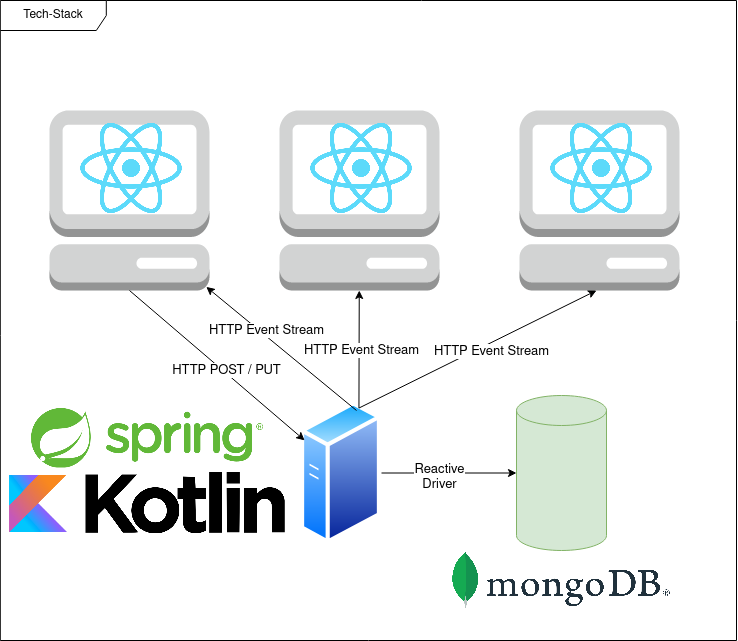
\includegraphics[width=\textwidth,height=\textheight,keepaspectratio]{TechStack}
    \caption{Technologie Stack}
\end{figure}
